\chapter{MeasSP}
Class to handle S--parameter measurement data, including bias
conditions, frequency range, etc.
\section{measSP}\hypertarget{measSP} %%%%%% MEASSP
Class constructor.
\subsection{Syntax}
\begin{verbatim}
    M = measSP
    M = measSP(A)
\end{verbatim}

\subsection{Description}
\verb"M = measmnt" returns a default measSP object including only information about when the object was created.\\
\verb"M = measmnt(A)", where \verb"M" is a measmnt object, returns a new measmnt object with same properties as \verb"A".\\
\subsection{Examples}
\begin{verbatim}
>> measSP
Measurement info
    Date : 17-Jul-2003 10:03:23
    Origin :
    Operator :
    Info :
Measurement state
    MeasType:   SP
Measurement Data
xparam-object
     type:  S
     reference: 50
     ports: 2
     elements:  0
\end{verbatim}
\subsection{Syntax}
\begin{verbatim}
    M = measmnt
    M = measmnt(A)
\end{verbatim}

%%%%%%%%%%%%%%%%%%%%%%%%% DISPLAY
\vspace{3mm} \hrule
\section{display}\hypertarget{measSP_display}
Display measSP object properties.
\subsection{Syntax}
\begin{verbatim}
    display(M)
\end{verbatim}

\subsection{Description}
\verb"display(M)" displays the non-empty properties of a measSP object. \\

%%%%%%%%%%%%%%%%%%%%%%%%% SET
\vspace{3mm} \hrule
\section{set}\hypertarget{measSP_set}
Set measSP object properties.
\subsection{Syntax}
\begin{verbatim}
    set(M)
    M = set(M,'P1',V1,'P2',V2,...)
\end{verbatim}

\subsection{Description}
\verb"set(M)" displays the non-empty properties and their values
of the measSP object \verb"M". \\
\verb"M = set(M,'P1',V1,'P2',V2,...)" assigns the the properties
\verb"'P1'" and \verb"'P2'" the values \verb"V2" and \verb"V2",
respectively. \verb"'P'" may also be \verb"measmnt",
\verb"measstate", or \verb"data" in order to assign the
corresponding measmnt, measstate, or xparam objects constituting
the measSP object.

\subsection{Examples}
\begin{verbatim}
>> M=measSP;
>> M=set(M,'Origin','C:\Measurements\FET.S2P')
Measurement info
    Date : 17-Jul-2003 10:06:06
    Origin : C:\Measurements\FET.S2P
    Operator :
    Info :
Measurement state
    MeasType:   SP
Measurement Data
xparam-object
     type:  S
     reference: 50
     ports: 2
     elements:  0
\end{verbatim}
The measstate properties of a measSP object may be directly
assigned:
\begin{verbatim}
>> m1=addprop(measstate,'MeasType','SP','Temp',150);
>> M=set(measSP,'measstate',m1)
Measurement info
    Date : 17-Jul-2003 10:14:22
    Origin :
    Operator :
    Info :
Measurement state
    MeasType:   SP
    Temp:   150
Measurement Data
xparam-object
     type:  S
     reference: 50
     ports: 2
     elements:  0
\end{verbatim}
\subsection{See Also}
\hyperlink{measSP_subsasgn}{measSP/subsasgn},
\hyperlink{measmnt_set}{measmnt/set},
\hyperlink{measmnt_addprop}{measmnt/addprop},
\hyperlink{measstate_set}{measstate/set},
\hyperlink{measstate_addprop}{measstate/addprop},
\hyperlink{measSP_get}{measSP/get}.

%%%%%%%%%%%%%%%%%%%%%%%%% GET
\vspace{3mm} \hrule
\section{get}\hypertarget{measSP_get}
Get measSP object properties.
\subsection{Syntax}
\begin{verbatim}
    v = get(M,'P1')
\end{verbatim}

\subsection{Description}
\verb"get(M)" returns the value of the \verb"M" property \verb"P1". \\

\subsection{Examples}
\begin{verbatim}
>> get(measSP,'Date')
ans =
17-Jul-2003 10:21:13

>> get(measSP,'data')
xparam-object
     type:  S
     reference: 50
     ports: 2
     elements:  0
\end{verbatim}
\subsection{See Also}
\hyperlink{measSP_subsref}{measSP/subsref},
\hyperlink{measSP_set}{measSP/set}.

%%%%%%%%%%%%%%%%%%%%%%%%% DELTA
\vspace{3mm} \hrule
\section{delta}\hypertarget{measSP_delta}
Returns the $\delta$-parameter of two-port S-parameters.
\subsection{Syntax}
\begin{verbatim}
    d = delta(M)
\end{verbatim}

\subsection{Description}
\verb"delta(M)" returns the $\delta$-parameter of the two-port S-parameters in \verb"M". \\

%%%%%%%%%%%%%%%%%%%%%%%%% FREQ
\vspace{3mm} \hrule
\section{freq}\hypertarget{measSP_freq}
Returns the measurement frequencies.
\subsection{Syntax}
\begin{verbatim}
    f = freq(M)
\end{verbatim}

\subsection{Description}
\verb"freq(M)" returns the frequencies of \verb"M".

\subsection{See Also}
\hyperlink{measSP_subsref}{measSP/subsref}.

%%%%%%%%%%%%%%%%%%%%%%%%% READ_TOUCHSTONE
\vspace{3mm} \hrule
\section{read\_touchstone}\hypertarget{measSP_read_touchstone}
Creates a measSP object from a Touchstone file.
\subsection{Syntax}
\begin{verbatim}
    msp = read_touchstone(M,'fname')
    msp = read_touchstone(M,'fname',N)
\end{verbatim}

\subsection{Description}
\verb"read_touchstone(M,'fname')" returns a measSP object created
from the measurement data in the Touchstone file \verb"fname".
Bias information etc. found in the file header are added to the
measSP object \verb"M" properties. By default, two-port
measurements are assumed. However, it may also be determined from
the file extension, i.e. \emph{fname.S3P} would determine
three-port
measurements.\\
\verb"read_touchstone(M,'fname',N)" specifies the numer of ports in \verb"N".\\

\subsection{Examples}
\begin{verbatim}
>> msp=read_touchstone(meassp,'ColdFET.s2p')
Measurement info
    Date : 2002-11-25, 11:36
    Origin :
    Operator :
    Info :
Measurement state
    MeasType:   SP
    Vgs:    0
    Vds:    0
    Igs:    -1.6283E-008
    Ids:    5.4435E-008
    Freq,min:   4.5E+007
    Freq,max:   2E+010
Measurement Data
xparam-object
     type:  S
     reference: 50
     ports: 2
     elements:  201
\end{verbatim}
\subsection{See Also}
\hyperlink{measSP_write_touchstone}{measSP/write\_touchstone},
\hyperlink{measSP_set}{measSP/set},
\hyperlink{measSP_subsref}{measSP/subsref}.

%%%%%%%%%%%%%%%%%%%%%%%%% WRITE_TOUCHSTONE
\vspace{3mm} \hrule
\section{write\_touchstone}\hypertarget{measSP_write_touchstone}
Write a measSP object to a Touchstone file.
\subsection{Syntax}
\begin{verbatim}
    write_touchstone(M,'fname')
\end{verbatim}

\subsection{Description}
\verb"write_touchstone(M,'fname')" writes the data stored into the
measSP object \verb"M" into the file '\emph{fname}'. If
\emph{fname} has no extension,
'\emph{.s2p}' is appended.\\

\subsection{See Also}
\hyperlink{measSP_read_touchstone}{measSP/read\_touchstone},
\hyperlink{measSP_set}{measSP/set},
\hyperlink{measSP_subsref}{measSP/subsref}.

%%%%%%%%%%%%%%%%%%%%%%%%% FMAX
\vspace{3mm} \hrule
\section{fmax}\hypertarget{measSP_fmax}
Maximum oscillation frequency.
\subsection{Syntax}
\begin{verbatim}
    d = fmax(M)
\end{verbatim}

\subsection{Description}
\verb"fmax(M)" returns the maximum oscillation frequency,
$f_{MAX}$, parameter from a two port device measurement stored
in the measSP object \verb"M". \\
\subsection{See Also}
\hyperlink{measSP_gtumax}{measSP/gtumax}.

%%%%%%%%%%%%%%%%%%%%%%%%% FT
\vspace{3mm} \hrule
\section{ft}\hypertarget{measSP_ft}
$f_T$ parameter for two port devices.
\subsection{Syntax}
\begin{verbatim}
    d = ft(M)
\end{verbatim}

\subsection{Description}
\verb"ft(M)" returns the extrapolated frequency where the
short-circuit gain of a two port, stored in the measSP object \verb"M", is unity. \\
\subsection{See Also}
\hyperlink{measSP_fmax}{measSP/fmax},
\hyperlink{measSP_h21}{measSP/h21}.

%%%%%%%%%%%%%%%%%%%%%%%%% GA
\vspace{3mm} \hrule
\section{ga}\hypertarget{measSP_ga}
The maximum available gain for two port devices.
\subsection{Syntax}
\begin{verbatim}
    d = ga(M)
\end{verbatim}

\subsection{Description}
\verb"ga(M)" returns the maximum available gain from a two port
device measurement stored in the measSP object \verb"M". \\
\subsection{See Also}
\hyperlink{measSP_gt}{measSP/gt},
\hyperlink{measSP_gtumax}{measSP/gtumax},
\hyperlink{measSP_gmsg}{measSP/gmsg},
\hyperlink{measSP_gp}{measSP/gp}.

%%%%%%%%%%%%%%%%%%%%%%%%% GMSG
\vspace{3mm} \hrule
\section{gmsg}\hypertarget{measSP_gmsg}
The maximum stable gain for two port devices.
\subsection{Syntax}
\begin{verbatim}
    d = gmsg(M)
\end{verbatim}

\subsection{Description}
\verb"gmsg(M)" returns the maximum stable gain from a two port
device measurement stored in the measSP object \verb"M". \\
\subsection{See Also}
\hyperlink{measSP_gt}{measSP/gt},
\hyperlink{measSP_gtumax}{measSP/gtumax},
\hyperlink{measSP_ga}{measSP/ga},
\hyperlink{measSP_gp}{measSP/gp}.

%%%%%%%%%%%%%%%%%%%%%%%%% GP
\vspace{3mm} \hrule
\section{gp}\hypertarget{measSP_gp}
The power gain for two port devices.
\subsection{Syntax}
\begin{verbatim}
    d = gp(M)
\end{verbatim}

\subsection{Description}
\verb"gp(M)" returns the power gain from a two port
device measurement stored in the measSP object \verb"M". \\
\subsection{See Also}
\hyperlink{measSP_gt}{measSP/gt},
\hyperlink{measSP_msg}{measSP/gmsg},
\hyperlink{measSP_gtumax}{measSP/gtumax},
\hyperlink{measSP_ga}{measSP/ga}.

%%%%%%%%%%%%%%%%%%%%%%%%% GT
\vspace{3mm} \hrule
\section{gt}\hypertarget{measSP_gt}
The transducer gain for two port devices.
\subsection{Syntax}
\begin{verbatim}
    d = gt(M)
\end{verbatim}

\subsection{Description}
\verb"gt(M)" returns the transducer gain from a two port
device measurement stored in the measSP object \verb"M". \\
\subsection{See Also}
\hyperlink{measSP_gp}{measSP/gp},
\hyperlink{measSP_msg}{measSP/gmsg},
\hyperlink{measSP_gtumax}{measSP/gtumax},
\hyperlink{measSP_ga}{measSP/ga}.

%%%%%%%%%%%%%%%%%%%%%%%%% GTUMAX
\vspace{3mm} \hrule
\section{gtumax}\hypertarget{measSP_gtumax}
The maximum unilateral transducer gain for two port devices.
\subsection{Syntax}
\begin{verbatim}
    d = gtumax(M)
\end{verbatim}

\subsection{Description}
\verb"gtumax(M)" returns the maximum unilateral transducer gain
from a two port device measurement stored in the measSP object \verb"M". \\
\subsection{See Also}
\hyperlink{measSP_gp}{measSP/gp},
\hyperlink{measSP_msg}{measSP/gmsg},
\hyperlink{measSP_gt}{measSP/gt},
\hyperlink{measSP_ga}{measSP/ga}.

%%%%%%%%%%%%%%%%%%%%%%%%% H21
\vspace{3mm} \hrule
\section{h21}\hypertarget{measSP_h21}
The short-circuit gain of a two port device.
\subsection{Syntax}
\begin{verbatim}
    d = h21(M)
\end{verbatim}

\subsection{Description}
\verb"h21(M)" returns the short-circuit gain from a two port device measurement
stored in the measSP object \verb"M". \\
\subsection{See Also}
\hyperlink{measSP_ft}{measSP/ft}.

%%%%%%%%%%%%%%%%%%%%%%%%% MASON
\vspace{3mm} \hrule
\section{mason}\hypertarget{measSP_mason}
Measure of activity of device. U = 1 is denoted fmax.
\subsection{Syntax}
\begin{verbatim}
    d = mason(M)
\end{verbatim}

\subsection{Description}
\verb"mason(M)" returns the Mason's gain from a two port device
measurement
stored in the measSP object \verb"M". \\
\subsection{See Also}
\hyperlink{measSP_h21}{measSP/h21}.

%%%%%%%%%%%%%%%%%%%%%%%%% K_FACT
\vspace{3mm} \hrule

\section{k\_fact}\hypertarget{measSP_k_fact}
The Rollet stability factor of a two-port device.
\subsection{Syntax}
\begin{verbatim}
    d = k_fact(M)
\end{verbatim}

\subsection{Description}
\verb"k_fact(M)" returns the Rollet stability factor for the two
port device measurement stored \verb"M". \\
\subsection{See Also}
\hyperlink{measSP_delta}{measSP/delta}.

%%%%%%%%%%%%%%%%%%%%%%%%% LENGTH
\vspace{3mm} \hrule

\section{length}\hypertarget{measSP_length}
The Rollet stability factor of a two-port device.
\subsection{Syntax}
\begin{verbatim}
    l = length(M)
\end{verbatim}

\subsection{Description}
\verb"length(M)" returns the number of measurement points,
normally frequencies, in \verb"M".

%%%%%%%%%%%%%%%%%%%%%%%%% SMITHPLOT
\vspace{3mm} \hrule

\section{smithplot}\hypertarget{measSP_smithplot}
Plot one or more two-port measSP objects in the Smith Chart.
\subsection{Syntax}
\begin{verbatim}
    smithplot(M)
    smithplot(M1,M2,...)
\end{verbatim}

\subsection{Description}
\verb"smithplot(M)" plots the two-port measSP objects in the Smith Chart. \\
\verb"smithplot(M1,M2,..)" allows several measSP objects to be plotted in the same Smith plot. \\

\subsection{Examples}
\begin{verbatim}
>> msp_cold=read_touchstone(meassp,'matlab_milou/test/cold.s2p');
>> msp_fwd=read_touchstone(meassp,'matlab_milou/test/forward.s2p');
>> smithplot(msp_cold,msp_fwd)
\end{verbatim}
Produces the following figure,\\
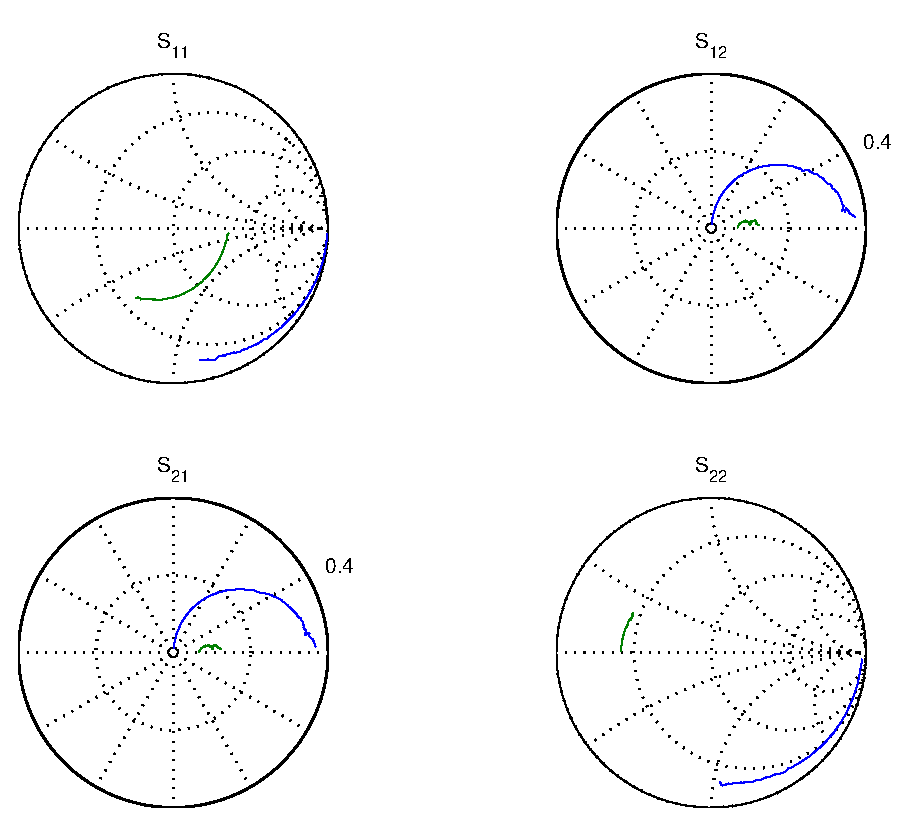
\includegraphics[width=8cm]{smith.eps}

%%%%%%%%%%%%%%%%%%%%%%%%% SUBSREF
\vspace{3mm} \hrule

\section{subsref}\hypertarget{measSP_subsref}
Overloads the subsref operator.
\subsection{Syntax}
\begin{verbatim}
    V  = M.P
    M2 = M(n)
\end{verbatim}

\subsection{Description}

%   V = M.P equals V = get(M,P)
%
%   M2 = M(f1) returns a new measSP object with the new frequency vector
%   defined from the f1 vector of new frequencies.

\verb"M.P" equals \verb"get(M,'P')" and provides a simple way of
extracting the values of an measSP object property.\\
\verb"M(n)" returns a new subset measSP object based on the
frequency indices in the vector \verb"n".

\subsection{Examples}
\begin{verbatim}
>> msp=read_touchstone(meassp,'matlab_milou/test/cold.s2p');
>> msp.Ids
ans =
  1.2009e-007

>> [msp.Freq/1e9 msp.S11]
ans =
   1.0000             0.9948 - 0.0325i
   1.4900             0.9940 - 0.0470i
   1.9800             0.9908 - 0.0644i
   2.4700             0.9908 - 0.0769i
   2.9600             0.9892 - 0.0916i
    ...
\end{verbatim}
The \verb"M(n)" indexing method:
\begin{verbatim}
>> msp(10:20)
Measurement info
    Date : 2002-10-25, 13:44
    Origin :
    Operator :
    Info :
Measurement state
    MeasType:   SP
    Vgs:    -1
    Vds:    0
    Igs:    -1.2426E-006
    Ids:    1.2009E-007
    Freq,min:   5.41E+009
    Freq,max:   1.031E+010
Measurement Data
xparam-object
     type:  S
     reference: 50
     ports: 2
     elements:  11
\end{verbatim}
\subsection{See Also}
\hyperlink{measSP_get}{measSP/get},
\hyperlink{measSP_set}{measSP/set},
\hyperlink{measSP_subsasgn}{measSP/subsasgn}.

%%%%%%%%%%%%%%%%%%%%%%%%% SUBSASGN
\vspace{3mm} \hrule

\section{subsasgn}\hypertarget{measSP_subsasgn}
Overloads the subsasgn operator.
\subsection{Syntax}
\begin{verbatim}
    M.P = V
\end{verbatim}

\subsection{Description}
\verb"M.P = V" equals \verb"M = set(M,'P',V)" and provides a
simple way for
changing the value of an measSP object property.\\

\subsection{Examples}
\begin{verbatim}
>> msp=read_touchstone(meassp,'matlab_milou/test/cold.s2p');
>> msp.Info = 'Assignment test'
Measurement info
    Date : 2002-10-25, 13:44
    Origin :
    Operator :
    Info : Assignment test
Measurement state
    MeasType:   SP
    Vgs:    -1
    Vds:    0
    Igs:    -1.2426E-006
    Ids:    1.2009E-007
    Freq,min:   1E+009
    Freq,max:   5E+010
Measurement Data
xparam-object
     type:  S
     reference: 50
     ports: 2
     elements:  101
\end{verbatim}
It can also be used to assign the S-parameters new values:
\begin{verbatim}
>> msp.S11 = rand(101,1);
\end{verbatim}
\subsection{See Also}
\hyperlink{measSP_subsref}{measSP/subsref}.

%%%%%%%%%%%%%%%%%%%%%%%%% INTERP
\vspace{3mm} \hrule

\section{interp}\hypertarget{measSP_interp}
Interpolate measurements.
\subsection{Syntax}
\begin{verbatim}
    M2 = interp(M,fsub)
    M2 = interp(M,psub,'P')
\end{verbatim}

\subsection{Description}
\verb"M2 = interp(M,fsub)" returns an object interpolated from the measSP object \verb"M" at the frequencies, \verb"fsub".\\
\verb"M2 = interp(M,psub,'P')" returns an object interpolated from the measSP object \verb"M" at property \verb"P" values \verb"psub".\\

\subsection{Examples}
\begin{verbatim}
>> msp=read_touchstone(meassp,'matlab_milou/test/cold.s2p');
>> msub=interp(msp,1e9:1e9:20e9)
Measurement info
    Date : 2002-10-25, 13:44
    Origin :
    Operator :
    Info :  Interpolated Freq.
Measurement state
    MeasType:   SP
    Vgs:    -1
    Vds:    0
    Igs:    -1.2426E-006
    Ids:    1.2009E-007
    Freq,min:   1E+009
    Freq,max:   2E+010
Measurement Data
xparam-object
     type:  S
     reference: 50
     ports: 2
     elements:  20
\end{verbatim}
\subsection{See Also}
\hyperlink{measSP_subsref}{measSP/subsref}.
